\documentclass{standalone}
\usepackage[dvipsnames]{xcolor}
\usepackage{tikz}
%\usepackage{pgfplots}
%\usepackage{pgfplotstable}
%\pgfplotsset{compat=1.5}
\usetikzlibrary{patterns}
\tikzstyle{proc1}=      [color=blue!20]
\tikzstyle{proc2}=      [color=blue!70]

\begin{document}
{
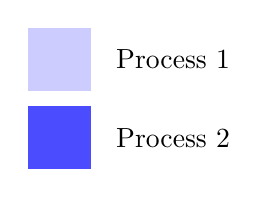
\begin{tikzpicture}
 \begin{scope}[yshift=-2cm]
  \fill[proc2] (0,0) rectangle (0.8,0.8);
  \node[right] at (1,0.4) {Process 2};
  \fill[proc1] (0,1) rectangle (0.8,1.8);
  \node[right] at (1,1.4) {Process 1};
 \end{scope}
\end{tikzpicture}
}
\end{document}
